% This example is meant to be compiled with lualatex or xelatex
% The theme itself also supports pdflatex
\PassOptionsToPackage{unicode}{hyperref}
\documentclass[aspectratio=1610, 10pt]{beamer}

% Load packages you need here
\usepackage{polyglossia}
\setmainlanguage{german}

\usepackage{csquotes}
    
\usepackage[style=numeric]{biblatex}
\addbibresource{lit.bib}

\usepackage{amsmath}
\usepackage{amssymb}
\usepackage{mathtools}

\usepackage{hyperref}
\usepackage{bookmark}

% load the theme after all packages

\usetheme[
  showtotalframes, % show total number of frames in the footline
]{tudo}

% Put settings here, like
\unimathsetup{
  math-style=ISO,
  bold-style=ISO,
  nabla=upright,
  partial=upright,
  mathrm=sym,
}

\title{Extending ctapipe image reconstruction using FACT methods}
\author[L Nickel/M.~Nöthe]{Lukas Nickel and Maximilian Nöthe}
%\institute[Kurzform Lehrstuhl]{Names des Lehrstuhls \\  Name der Fakultät}
%\titlegraphic{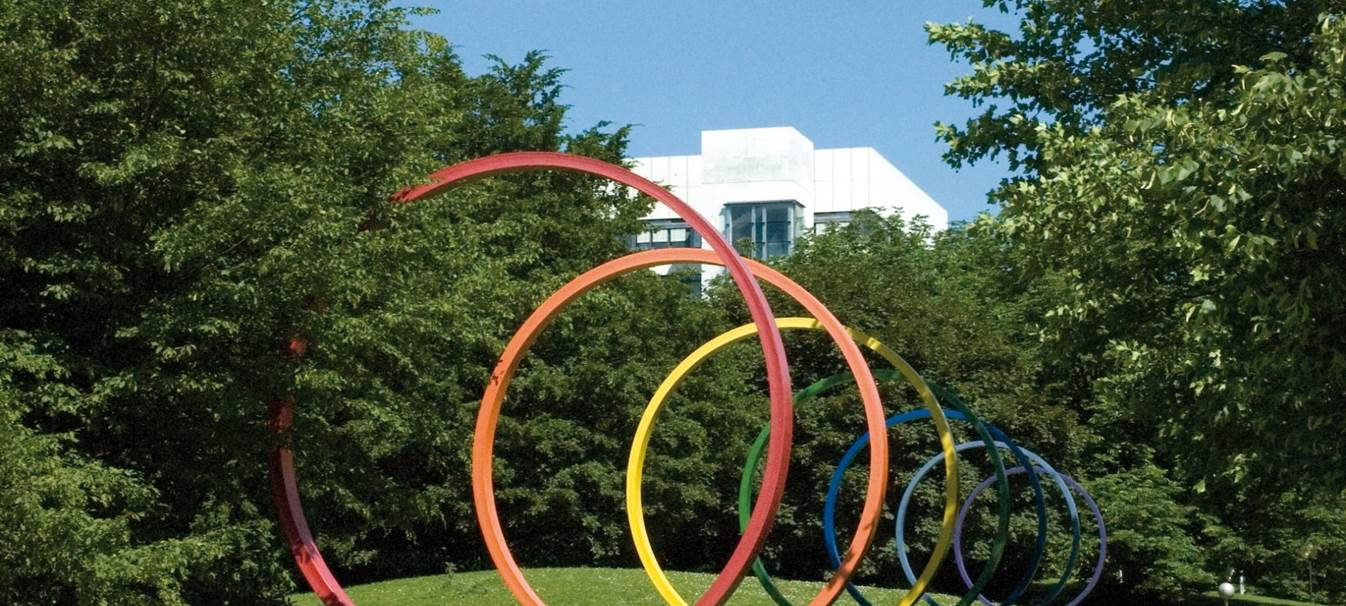
\includegraphics[width=0.7\textwidth]{images/tudo-title-2.jpg}}


\begin{document}

\maketitle

\begin{frame}{Overview}
 \begin{itemize}
    \item {\Large What is CTA?}

    Taking stereoscopic reconstruction to the extreme:
    The Cherenkov Telescope Array.
    \vspace{20pt}

    \item {\Large Progress of ctapipe}

    How is CTA data going to be handled?
    ctapipe: A low-level data processing pipeline software for CTA.
    \vspace{20pt}

    \item {\Large What can we learn from FACT?}
    
    The First G-APD Cherenkov Telescope:
    Transfering knowledge from single telescope analysis.
    

 \end{itemize}
\end{frame}

\begin{frame}
    - was ist cta?
    - was ist geplant?
    - was ist fertig?
    - womit können wir arbeiten?
    - status MC
    - was ist ctapipe?
    - wie soll es funktionieren? low-level-kram -> ? daten level? dl0,dl1,...?
    - status ctapipe
\end{frame}

\begin{frame}{column test}
    \begin{columns}[T] % align columns
        \begin{column}{.48\textwidth}
            \color{red}\rule{\linewidth}{4pt}
            \begin{enumerate}
                \item "Cherenkov Telescope Array"
                \item Proposed in 2005, currently in pre-production
                \item Two arrays of multiple telescopes (>100) instead of single telescopes
                \item Goals: Extend observable energy range(20GeV-300TeV), huge field of view()
                \item Status: First light on LST and Schwarzschildt-Couder-Telescope
            \end{enumerate}
        \end{column}%
        \hfill%
        \begin{column}{.48\textwidth}
            \color{blue}\rule{\linewidth}{4pt}
            \begin{figure}
                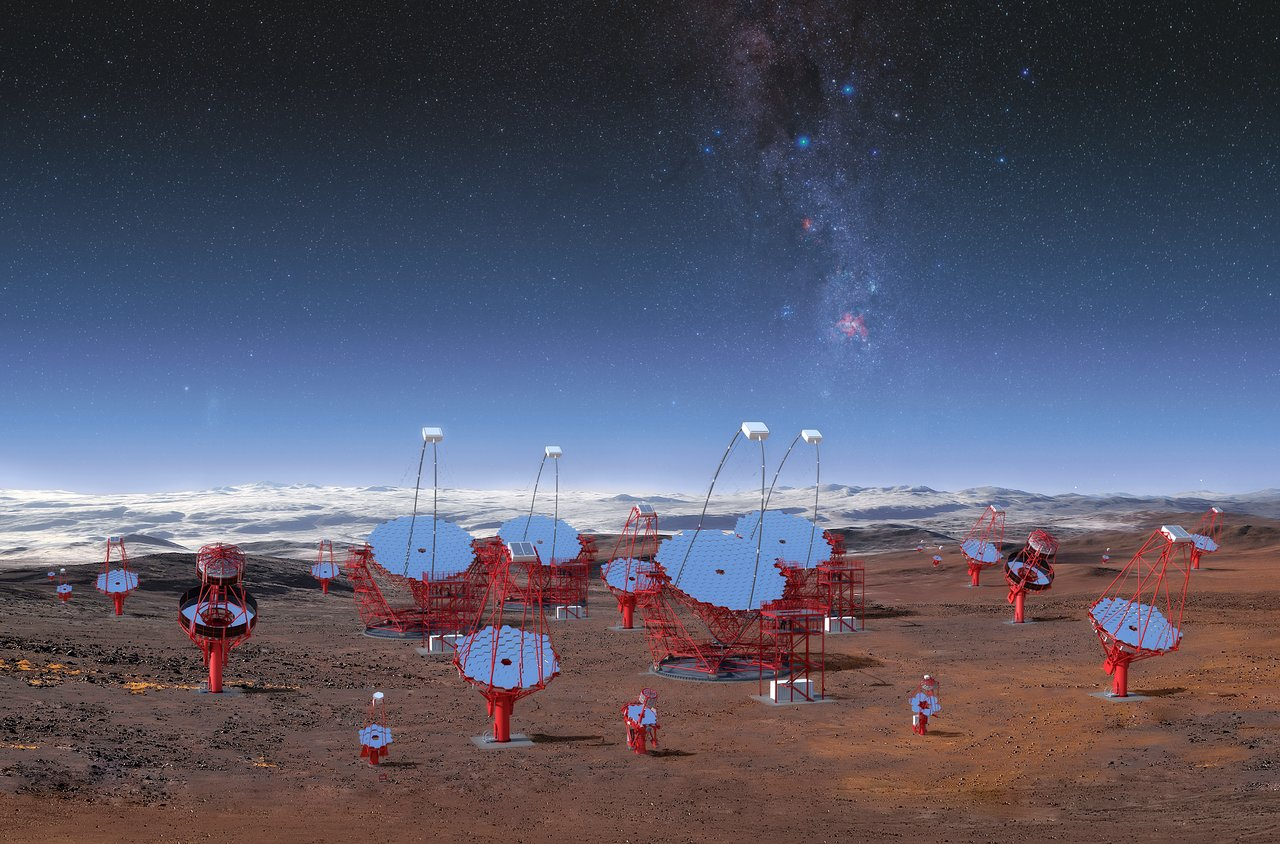
\includegraphics[width=\linewidth]{images/cta_telescopes.jpg}
                \caption{Visualization of the different telescope types. Credit: CTA/M-A. Besel/IAC (G.P. Diaz)/ESO}
            \end{figure}
        \end{column}%
    \end{columns}
\end{frame}


\begin{frame}{Expected sensitivity}
    \begin{figure}
        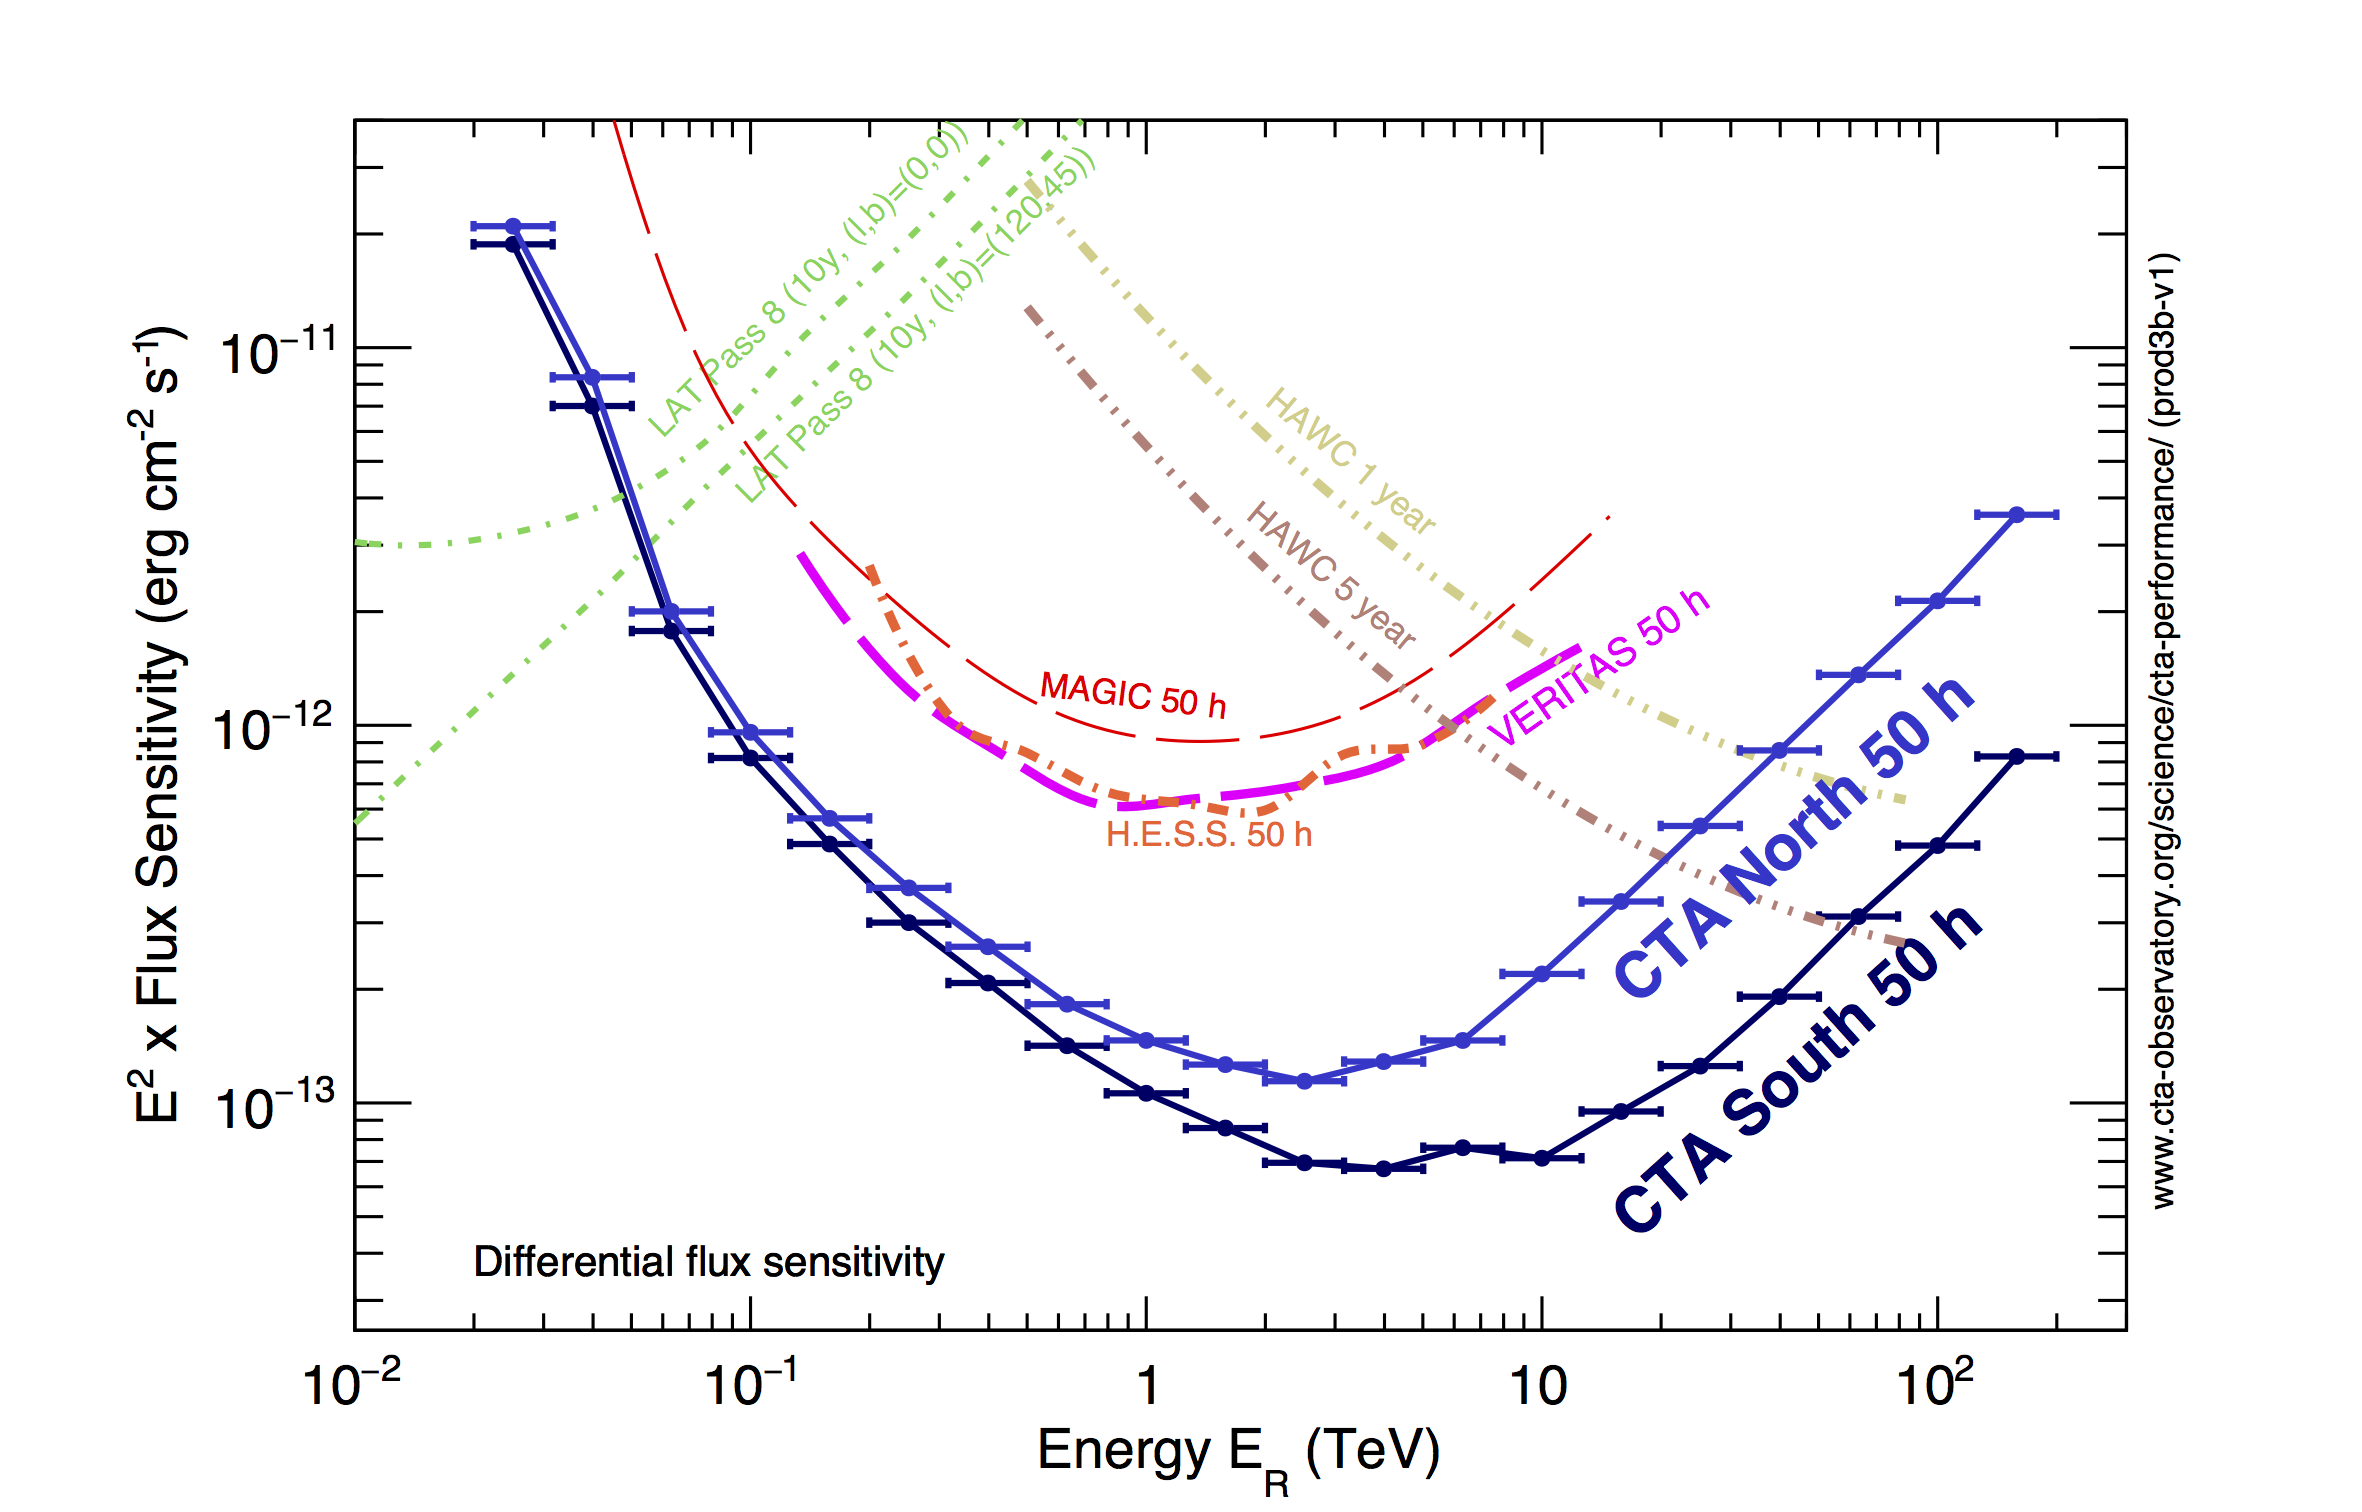
\includegraphics[width= 0.8\linewidth]{images/cta_sensitivity.png}
        \caption{Credit: CTA/M-A. Besel/IAC (G.P. Diaz)/ESO}
    \end{figure}

\end{frame}

\begin{frame}{ctapipe}
    \begin{enumerate}
        \item low level pipeline for cta data
        \item calibration, cleaning, hillas, ...
        \item in development, prototype
        \item python based
        \item ??
    \end{enumerate}
\end{frame}

\section{Adding FACT to the mix}

\begin{frame}{The FACT experiment}
    \begin{columns}[T] % align columns
        \begin{column}{.45\textwidth}
            \vspace{10pt}
            \begin{itemize}
                \item "First G-APD Cherenkov Telescope"
                \item Operating in La Palma since 2011
                \item Monoscopic reconstruction only
                \item What did we take a look at?
                \begin{itemize}
                    \item{More advanced cleaning method}
                    \item{Distinction of "islands" in shower images}
                    \item[\rightarrow] Possible improvements for monoscopic reconstruction in ctapipe
                    \item[\rightarrow] First use case: LST1
                \end{itemize}
            \end{itemize}
        \end{column}
        \begin{column}{.48\textwidth}
            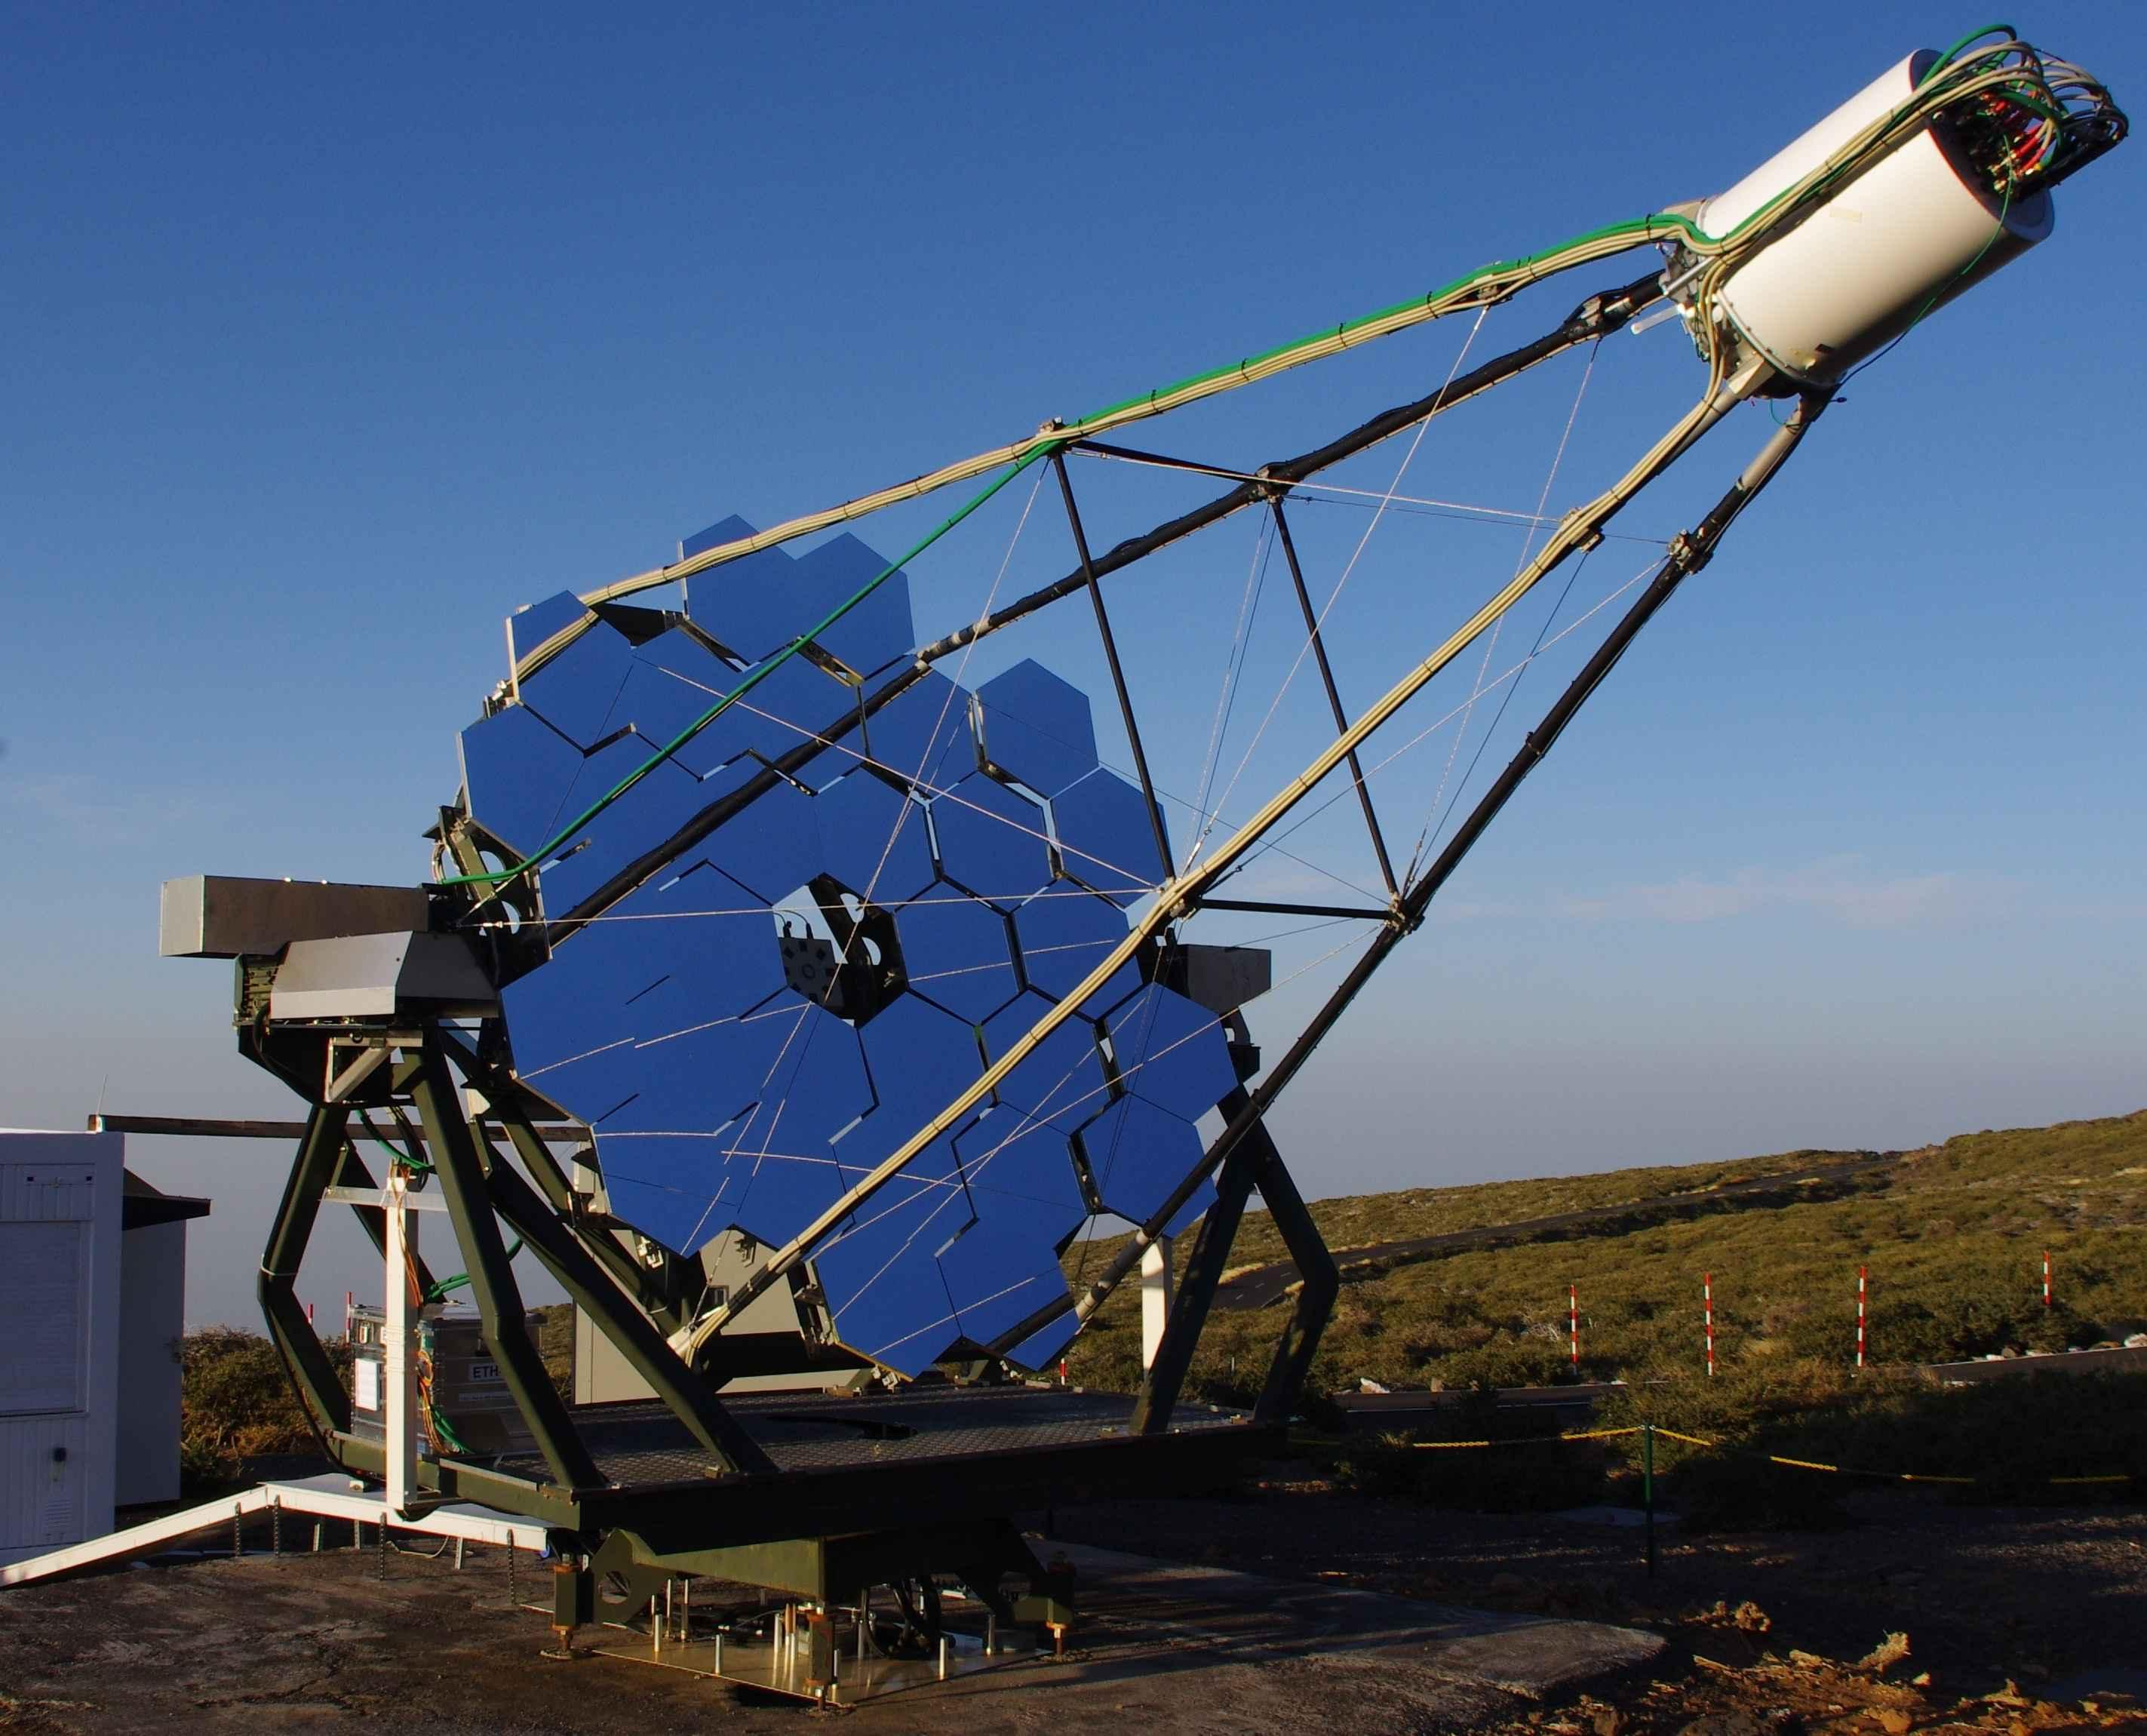
\includegraphics[width=\linewidth]{images/fact_telescope.jpg}
            \cite{Anderhub_2013}
        \end{column}
    \end{columns}
\end{frame}

% \begin{frame}{Why does it matter?}
%     \begin{itemize}
%         \item Knowledge in developing a processing pipeline 
%         \item Possible improvements for CTA single telescopes
%         \item More advanced cleaning
%         \item Distinction of "islands" in shower images
%     \end{itemize}
% \end{frame}
% \begin{frame}
%     - was ist tailcuts?
%     - wo liegt der unterschied? -> besonders zeitkomponente
%     - ist die schon richtig drin in cta?
%     - cleaning level von tailcuts ableiten
%     - vergleich auf schauerbildern
%     - extremfälle: was bringt das?
%     - Effekt auf ML
% \end{frame}

\section{Alternative cleaning method}
\begin{frame}{Cleaning methods}
    \begin{columns}[T] % align columns
        \begin{column}{.48\textwidth}
            Tailcuts Cleaning
            \begin{enumerate}
                \item "two treshold procedure"
                \item pixels above t1 will be kept
                \item neighboring pixels above t2 will be kept
                \item "lonely" pixels wont survive
            \end{enumerate}
        \end{column}
        \begin{column}{.48\textwidth}
            FACT image cleaning
            \begin{enumerate}
                \item similar behaviour, but also uses information about the arrival times
                \item pixels with a very different arrival time than their neighbours get removed
                %\item for now arrival times are integers in ctapipe -> limits search for optimal threshold
                \item removes "lonely" pixels multiple times
                \item one would assume less separated pixels
                \item intensity threshold should probably be a bit more loose than with tailcuts
        \end{enumerate}
        \end{column}
    \end{columns}
\end{frame}

\begin{frame}{timing information}
    \begin{figure}
        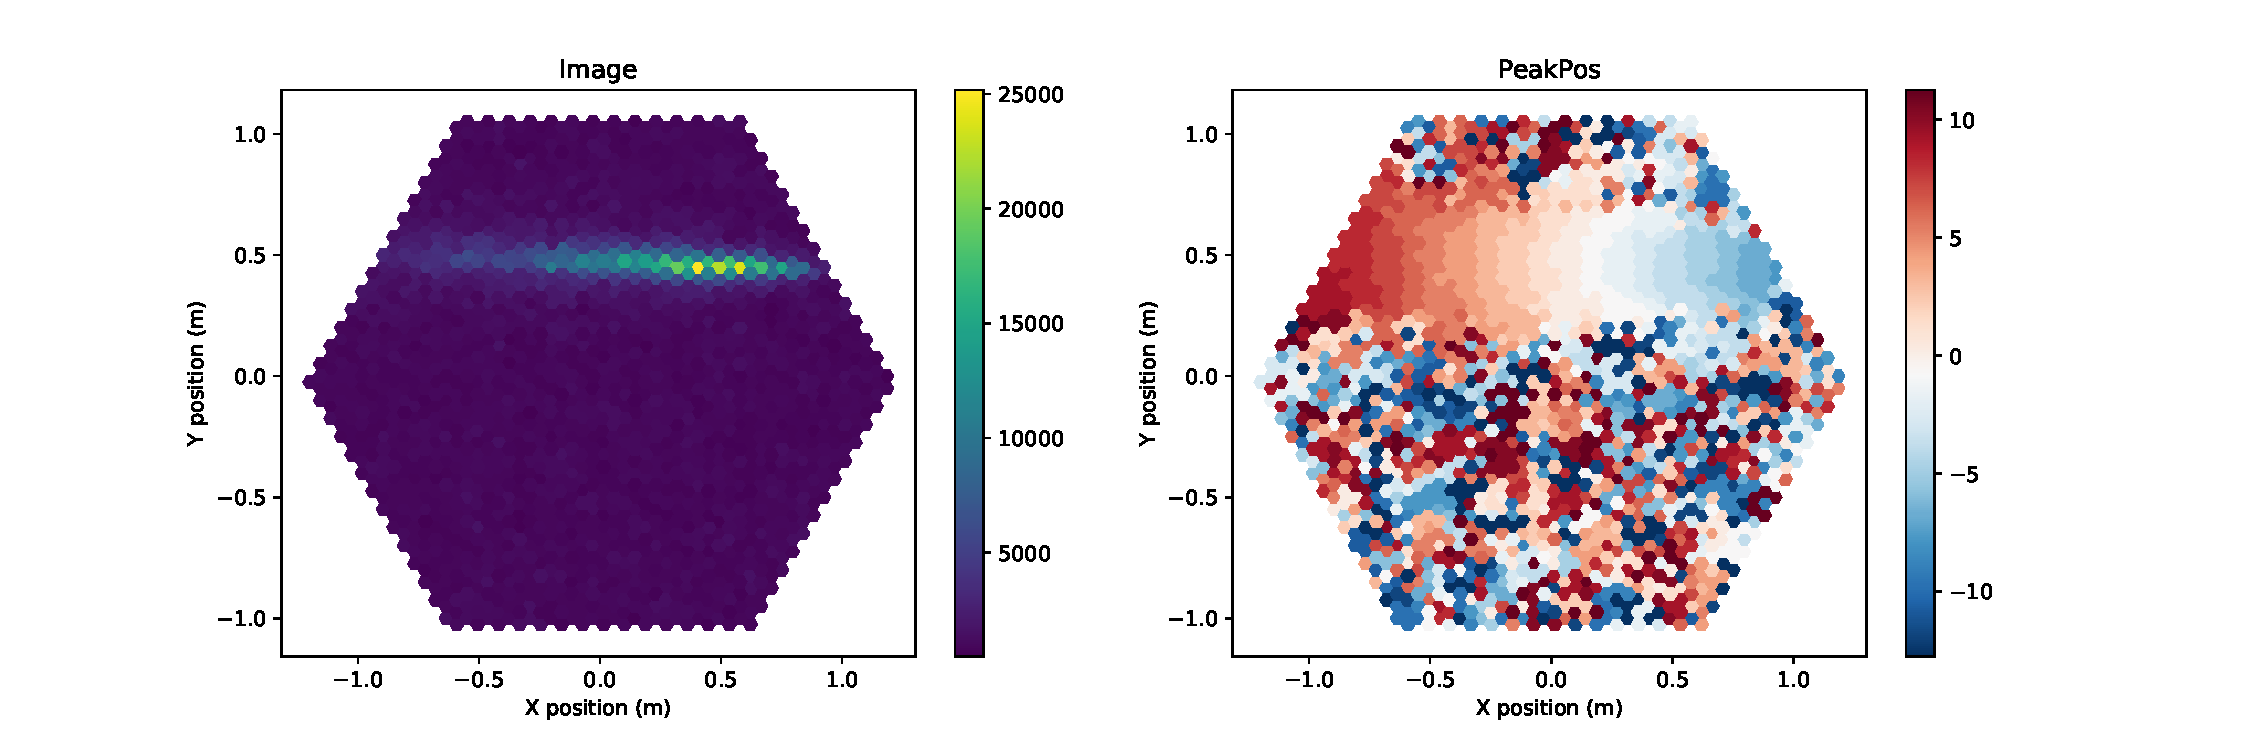
\includegraphics[width=\linewidth]{images/peakpos.pdf}
    \end{figure}
    Intensity and relative arrival time for a MC gamma-event
\end{frame}


\section{Finding islands}

\begin{frame}
    \centering
    {\Huge \textbf{Finding islands}}
\end{frame}

\begin{frame}{A well cleaned gamma event}
    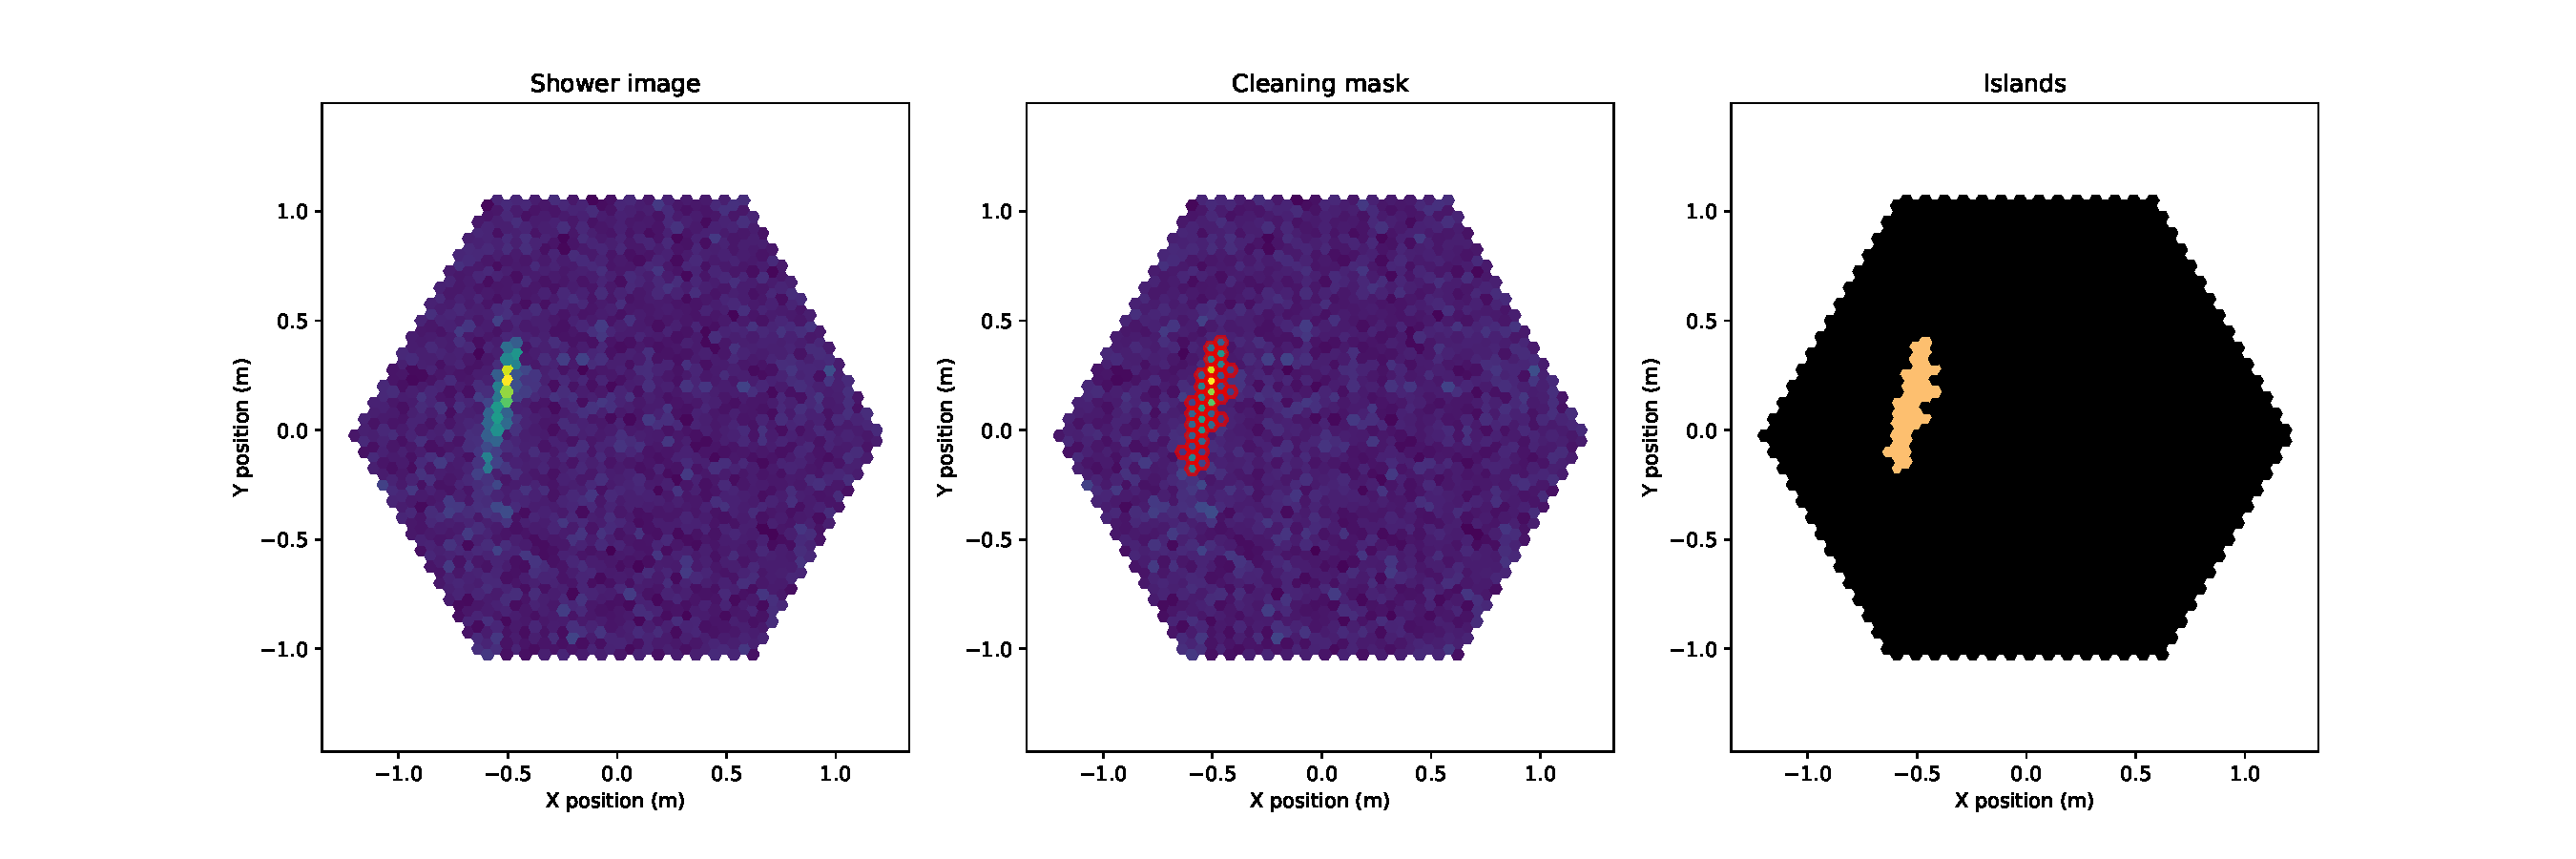
\includegraphics[width=\linewidth]{images/islands_single.pdf}
\end{frame}


\begin{frame}{Our poorly cleaned sample event}
    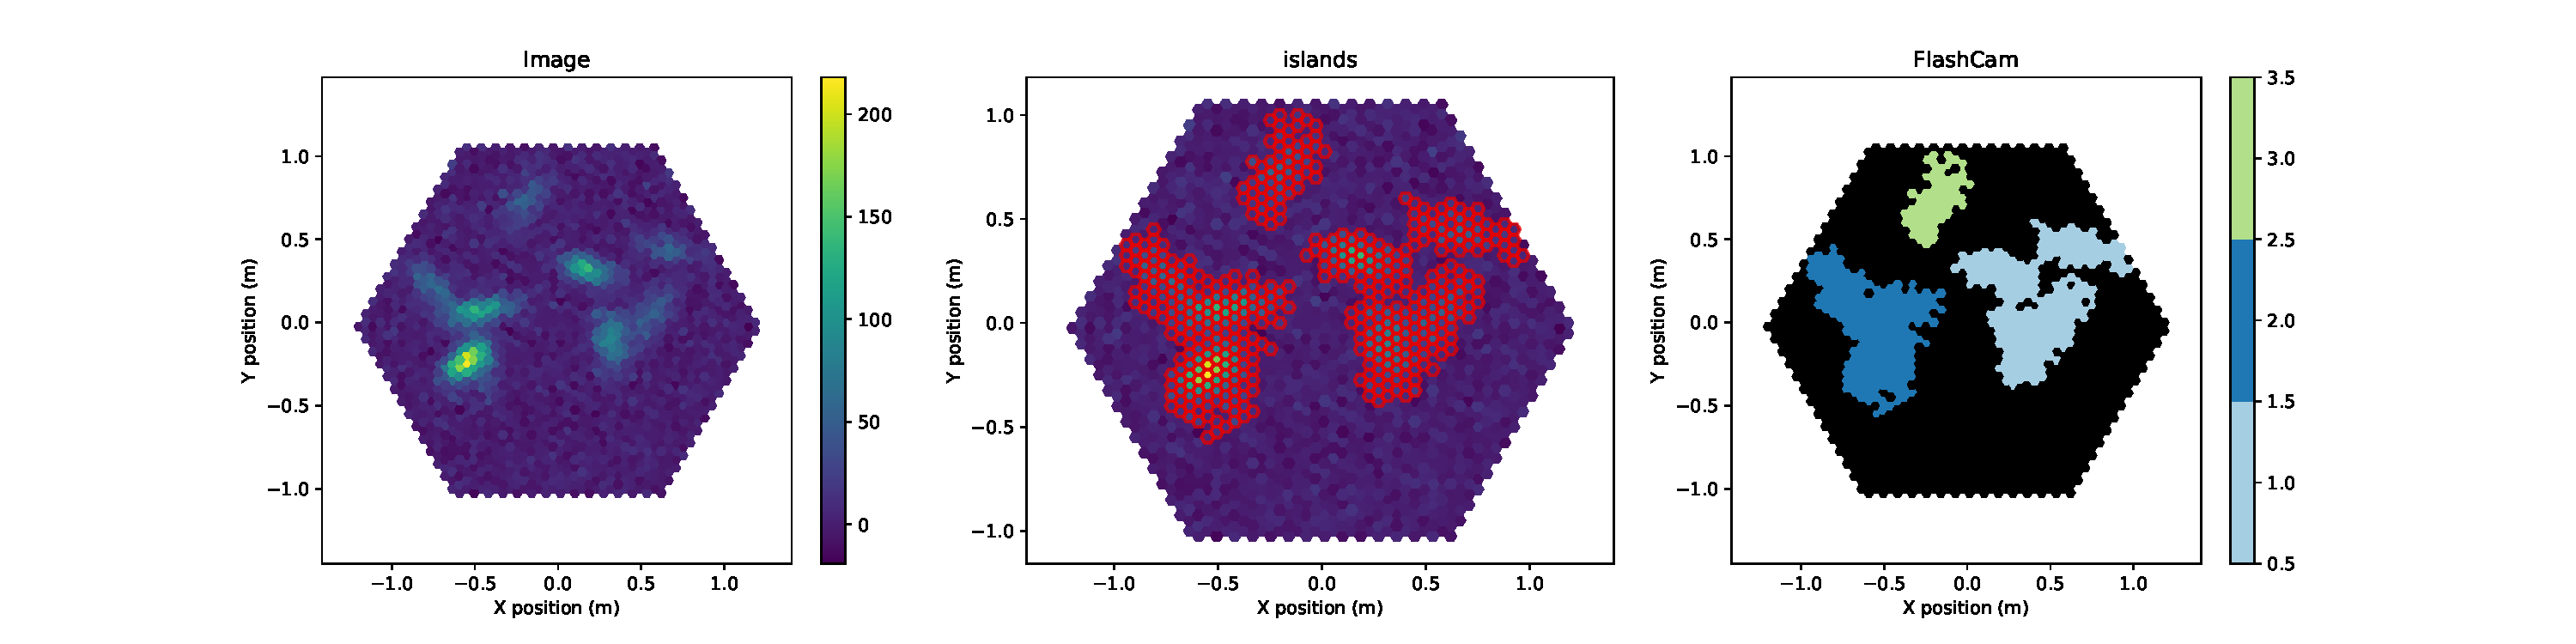
\includegraphics[width=\linewidth]{images/islands.pdf}
\end{frame}


% vlt besser je config die ergebnisse?

\section{Comparison}
\begin{frame}{g/h separation}
    erklären

    bild von verschiedenen configs
\end{frame}

\begin{frame}{energy regression}
    erklären

    bild von verschiedenen configs
\end{frame}

\begin{frame}{islands}
    mit einer config vergleichen (oder 2: tailcut und beste fact config)
\end{frame}

\printbibliography
\end{document}
